
\section{Mini-batch 在 SGD 中的应用}


\subsection{Pytorch 中使用 mini-batch 加速 RNN 训练}

%

%%
%
\subsection{mini-batch 的 group 算法}


Accelerating Recurrent Neural Network Training using Sequence Bucketing and
Multi-GPU Data Parallelization\cite{}

\subsection{用 mini-batch 加速 Tree-LSTM}

\subsubsection{iprally}

https://www.iprally.com/news/the-worlds-fastest-tree-lstm

The world’s fastest Tree-LSTM, Sept 5, 2018,
www.iprally.com 公司的一篇blog.
大致是 拓扑排序后 mini batch的 tree-LSTM. 按照 tree node 的深度排序.

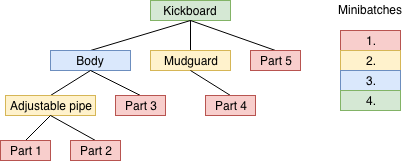
\includegraphics[width=0.6\linewidth]{pytorch/pic/minibatch_order.png}

\subsubsection{nicolaspi}

Tensorflow 上的类似工作,
https://github.com/nicolaspi/treelstm, March 2017.

This implementation builds a meta-tree per minibatch that aggregates all its
samples. A meta-tree is then processed heightwise. Each nodes with a given
height h depends only from nodes of height h-1, this allows to aggregate all
matrix mutliplications within h. Thus the number of matrix multiplication per
mini batch can be reduced from O(MxN) to O(log(N)) where M is the mini batch
size and N the number of nodes. The result is a training time 70x faster with
the reference model : https://github.com/sapruash/RecursiveNN.

和 iprally 一样按照节点的深度排序.

\subsubsection{Nvidia}
Nvidia 的一篇博客, April 9, 2017,
\href{https://devblogs.nvidia.com/recursive-neural-networks-pytorch/}
{Recursive Neural Networks with PyTorch}



